\section{Programmbeschreibung}\label{programm}

% Problemstellung/Fragestellung:
Die Anwendungssoftware „Flower Segmentation Tool“ wurde zur Erkennung von Arnica montana durch die Auswertung von Drohnenluftbildern entwickelt. Ziel ist es das Monitoring von Arnica montana durch eine nachhaltige Pflückung auf bisher nicht genutzte Flächen auszuweiten. Durch den Drohneneinsatz können auch in unwegsamen Gelände Erkenntnisse über den Bestand von Arnika gewonnen werden. Als Datengrundlage bei der Entwicklung dienten die Aufnahmen der Testflüge aus dem Schwarzwald des „Projekt zum Schutz der Biodiversität in Rumänien“.
Das „Flower Segmentation Tool“ ist so konzipiert, dass schnelle Berechnungen Aussagen über den Bestand getroffen werden können, die dann vor Ort weiter untersucht werden. Es soll also unterstützend zur Feldarbeit wirken und dabei eine Einschätzung liefern, wo diese stattfinden kann. 
%Anforderungen an den Code
Die wichtigste Anforderung an das Programm ist dabei trotz großer Datenmengen noch in angemessener Schnelligkeit zu agieren. Um eine einfache Installation zu ermöglichen, wurde darauf geachtet niedrigschwellige Soft- und Hardwarevoraussetzungen zu fordern. 
%Anforderungen an die Benutzeroberfläche
Die Grafische Benutzeroberfläche besteht aus zwei Teilen. Einerseits soll die grafische Darstellung der Bilder zum Ausprobieren der Parameter möglich sein. Dabei ist ein vielseitiger Plotfenster mit der Möglichkeit den Ausschnitt zu verändern und Teile des Bildes zu vergrößern eine wichtige Funktion. Andererseits soll eine einfacher Anwendung der Berechnung auf einen großen Datensatz möglich sein. Bei beiden Anwendungen soll eine Statusanzeige einen Überblick verschaffen, welche Prozesse im Hintergrund laufen.

\subsection{Programmiersprache}
Python ist eine Open Source Programmiersprache, die plattformübergreifend auf allen gängigen Betriebssystemen anwendbar ist. Die interpretierte Skriptsprache wurde 1994 von dem niederländischen Programmierer Guido Rossum als Python 1.0 veröffentlicht. Der Name Python hat Rossum von der britischen Komikergruppe Monty Python abgeleitet.
Entscheidener Unterschied zu anderen höheren Programmiersprachen, ist der gut lesbare und knapp gehaltene Stil von Python. Ziel ist es Redundanz zu vermeiden und Übersichtlichkeit zu optimieren. Zur Strukturierung verwendet Python Einrückungen und kommt mit wenigen Schlüsselwörtern aus. Mit diesem reduzierten Syntax schafft Python Einfachheit, ohne dabei eine Komplexität zu verhindern. Python unterstützt objektorientierte und funktionale Programmierung. Es gibt eine umfassende  Standartbibliothek und zusätzlich die Möglichkeit der Erweiterung einer Vielzahl an Modulen, die in den Skripten import werden können.
%Vielzahl von NutzerInnen (kommerziell, wissenschaftlich, Betriebssystemen, Webframeworks)

%- Python-Interpreter, die stärksten sind CPython, basiert auf der Programmiersprache C und Jython basierend auf Java. 
%-  Compiler, die Python in andere Programmiersprachen übersetzten und dort nutzbar machen.

Seit 2001 wird Python durch die Python Software Foundation stetig weiterentwickelt. 
Python 2 gibt es seit 2000, Python 3 seit 2008. Dies beinhaltet so tiefgreifende Änderungen, dass einige Funktionen, die unter Python 2 geschrieben wurden, nicht mehr unter Python 3 funktionieren würden. Deshalb wird Python 2.7 noch bis Ende 2019 mit weiteren Updates unterstützt. Die aktuellste stabile Version ist seit 2018 Python 3.7 \citep[vgl.][]{PSF2019}.

%Verweis auf Einstiegsmöglichkeit in die verwendete Programmiersprache-> Anhang

%Verwendete Pakete???
\subsection{Anwendungsbereich} %Zusammenfassung Anwendungsmöglichkeiten des Programms
Das Programm soll zur Bildanalyse und Auswertung von Luftaufnahmen, die von Drohne aufgenommen wurden, angewendet werden. Es können RGB Fotos eingelesen und analysiert werden. Da bei der 
Es werden aus RGB Fotos die gelben Farbebereiche angezeigt. Diese können in der Größe beschränkt werden. Auf verschiedene Arten können so gelbe Blumen im Bild erkannt und das Ergebnis auf verschiedene Weise angezeigt werden. Der User? kann die Parameter selbst festlegen und sich das Ergebnis im Plotfenster ansehen, heran zoomen, Parameter anpassen. Die Berechnung kann auf einzelne Bilder angewendet und diese dann exportiert werden, oder auf alle Bilder eines Ordners, und so große Datenmengen mit einem Aufruf? verarbeitet werden. 

% Einordnung in die "Aufgabe des Programms" für das Projekt???
%genaue Funktionen (zentrierter Crop, Bilder plotten lassen, exportieren, segmentieren, circles, dabei größe anpassen)
\subsection{Programmaufbau}
(Flow-chart und Beschreibung der einzelnen Bestandteile und der Verknüpfungen zwischen den Modulen)
     - Modulübersicht (Folderstruktur)
    
    - Flow-Chart von einem Beispiel wie das Bild bearbeitet wird, en detail

\begin{figure}[htb]
 \centering
 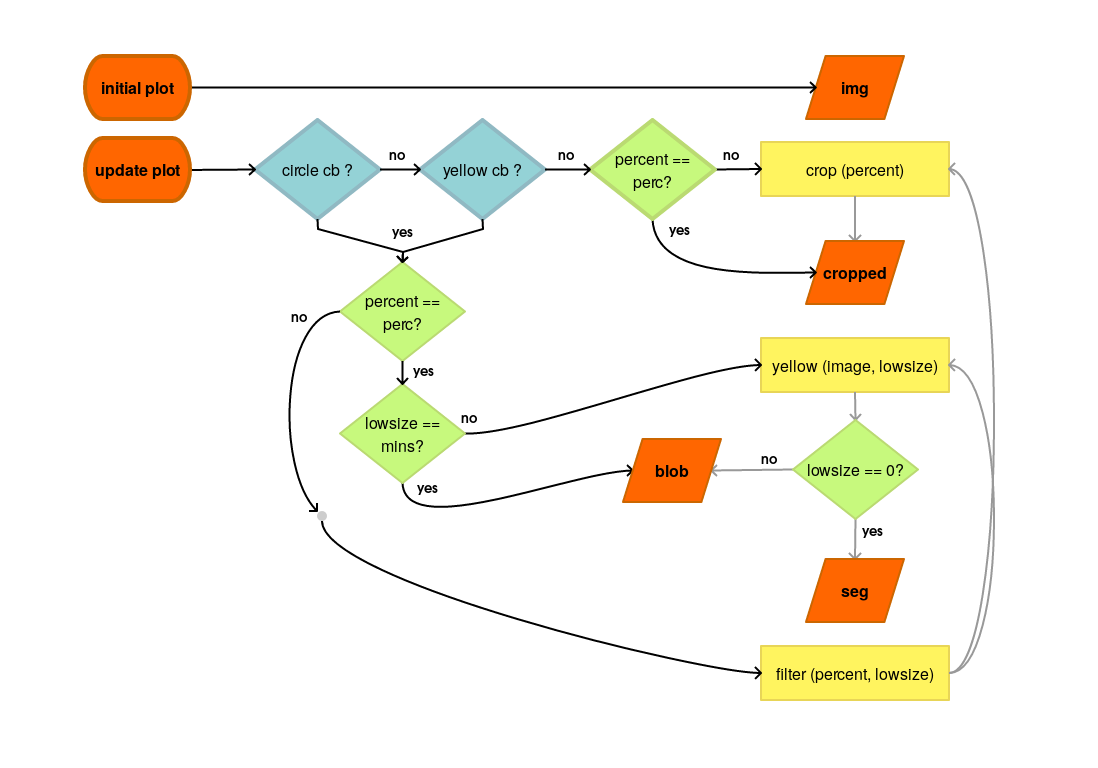
\includegraphics[width=\textwidth,angle=0]{abb/prozess-flow}
 \caption{Programm flowchart}
\label{fig:flowchart}
\end{figure}

Die inneren Prozesse einer Plotabfrage werden in Abbildung \ref{fig:flowchart} (S.\pageref{fig:flowchart}) dargestellt. Hauptintention dabei stellt die Minimierung von Zeitverzögerungen da. Vor Allem die Wiederholung von unnötigen Berechnungen soll durch if-else Schleifen vermieden werden. Es werden je nach Prozess der berechnet wird zunächst erstmal abgefragt, ob sich die Parameter überhaupt verändert haben. 
Ist dies nicht oder nur teilweise der Fall kann eine erneute komplette Berechung nicht notwenig sein und der angefragte Prozess auf ein schon gespeichertes Bild oder eine Teilfunktion direkt zurückgreifen kann. Der Aufruf des Gesamtfilters, der die gelben Bildteile mit einer Mindestgröße segmentiert, ruft Funktionen auf, die jeweils auch direkt von anderen Anfragen angesprochen werden können. Dabei werden die Zwischenergebnisse als Objekte der Klasse gespeichert. Insgesamt kann so die Ausgabe effizienter und schneller wiedergegeben werden, gerade bei Bilder, die eine große Dateimenge einnehmen.

\subsection{Vorgehensweise Methoden?}

genaue Beschreibung der Methoden (Wie wird der Bereich heraus gefiltert, Datenstruktur?, GUI, Parameter)
nach welchen Kriterien und warum diese gewählt -> Quellen?

Methoden: 
- Filtern nach Farbebereich -> liegt der Bildpunkt nicht in dem Bereich wird ihm 0 zugeordnet, sonst 255. So entsteht eine Maske des Bildes mit allen gelben Bereichen.
Diese kann wieder auf das original Bild übertragen werden. 
% dafür wird das Bild als dreidimensioneller BGR-Array mit je einer Ebene je Farbband. Mit der Funktion cv2.inRange() wird eine Maske erstellt, die für alle Pixel, die nicht in dem Bereich sind 0 zuordnet und für alle die in dem Bereich sind 255. Diese Maske lässt sich auf das originale Bild mit cv2.bitwise() übertragen. Dabei werden zwei Bilder zusammengefügt, im Bereich einer Maske.??doppelt?? 
Warum nach Farbbereich filter:

\subsubsection{Parameterbeschreibung}


\subsection{Implementierung / Aufruf}    
- Flow-Chart für die GUI und den Programmaufruf, quasi als "Anleitung der Benutzung"
\subsubsection{Hard- und Softwarevoraussetzungen}
\subsubsection{(Notwendige) In- und Output-Dateien und deren Formate}



- Einbindungsmöglichkeiten in andere Anwendungen
- Bei komplexen Berechnungsverfahren Beschreibung der Algorithmen und Literaturhinweise zu den Quellen der Verfahren


    
